% $Id$

\chapter{System Execution Trace Adaptation Framework (SETAF)}
\label{chap:setaf}

This chapter discusses a tool and a method called \textit{System 
Execution Trace Adaptation Framework (SETAF)} in the CUTS  analysis 
tool set. This tool is used as an extension to UNITE when analyzing QoS 
properties from system execution traces.

\section{Overview}
\label{sec:setaf-overview}

Chapter~\ref{chap:unite} discussed the method of UNITE when doing the 
QoS analysis using system execution traces. In some situations UNITE cannot 
be used alone to analyze system execution traces. This is because UNITE 
assumes that every different instance of a log format is unique. Which means 
it assumes that at least one log format variable other than the variable represent 
time have different values among different instances. This causes non-unique 
relations among different instances of log formats.

\begin{lstlisting}[label=listing:trace2, 
caption=Portion of a system execution trace that does not 
contain unique relations ., captionpos=b]
      Started doing task A at 12.00
      Finished doing task A at 12.01
      Started doing task A at 12.02
      Finished doing task A at 12.03
\end{lstlisting}

For example, Listing~\ref{listing:trace2} illustrates 
an example system execution trace where the dataflow graph
will not have unique relations between the log format. This 
is because it is \textit{hard} to know start/finish messages 
are associated with one another without human intervention.
Moreover, when an example similar to the one present in 
Listing~\ref{listing:trace2} is analyzed by UNITE, it 
will yield incorrect results because it is \textit{hard} to 
determine correct causality between similar log messages.

With proper planning early in the software lifecycle, it is
possible to ensure generated system execution traces have unique
relations to facilitate proper analysis. This, however, is not
alway possible---especially when analyzing system execution traces
generated by third-party systems and their components. Although
such system execution traces may not contain unique 
relations, the existing relations can be exploited (or adapted) 
to enforce a unique relation. For example, in 
Listing~\ref{listing:trace2}, although the relation is 
not unique, it can be adapted to be a unique relation by adding 
an id to each log message. This will ensure that UNITE analyzes 
the dataflow model and evaluates the expression correctly. 

Adding this kind of new ids means we have to add new log format 
variables to the identified log formats. Further new log format relations 
need to be identified for these newly added variables. Even though 
the ordinary log format variables get values from the system execution trace, 
it does not contain the values for these externally added log format 
variables.  Further the variables need to be added, the relations need 
to be enforced and what sort of values they get depend on the system 
execution trace being analyzed. Therefore UNITE provides a common 
interface for these task, but the implementation module should take 
care of how to adapt the dataflow model. Distributed system testers 
need to find out the adaptation patterns and need to provide these 
external adapters. 

Distributed system testers do not need to develop 
these modules using a language like C++. 
Instead SETAF provides a simple language 
to specify them as a adaptation specification. SETAF has a code 
generation tool to generate the source code for these adapters. After 
compiling these adapter modules, they need to be specified in the 
datagraph file so that UNITE can load them during the run time. The 
Figure~\ref{fig:setaf} showcase the overall workflow of SETAF.

\begin{figure}[htbp]
  \centering
  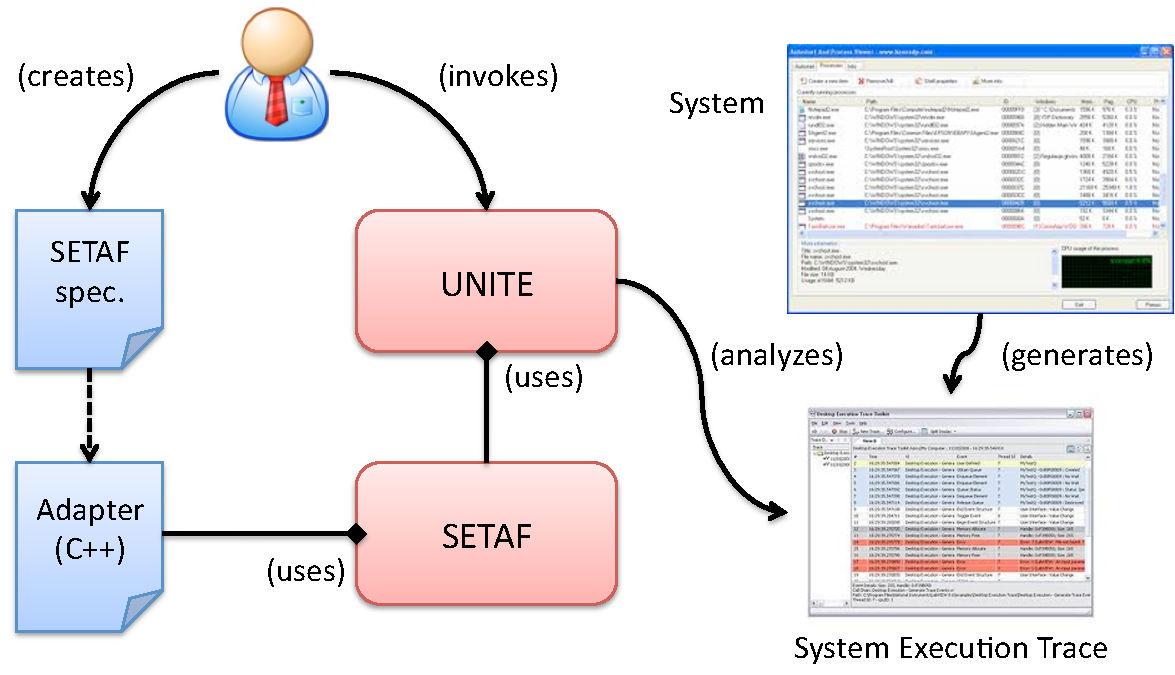
\includegraphics[scale=0.7]{analysis/setaf.pdf}
  \caption{Conceptual overview of SETAF's workflow.}
  \label{fig:setaf}
\end{figure}

The rest of the chapter describes the content of the UNITE Adapter 
Specification in Section~\ref{sec:unite-uas}. In Section~\ref{sec:code-gen} 
it describes the procedure of code generation of adapter modules in SETAF.
Finally Section~\ref{sec:qos-analysis} shows how to use SETAF with 
UNITE to do the QoS analysis. 

\section{UNITE Apater Specification}
\label{sec:unite-uas}

This section explains the content of Unite Adapter Specification. Listing
~\ref{listing:example.uas} shows an example of UNITE Adapter specification. 

\lstinputlisting[label=listing:example.uas,
  caption=An example UNITE Adapter Specification.,
  captionpos=b,numbers=left]{analysis/example.uas}


As shown in the listing the UNITE Adapter Specification has five sections (
\texttt{Variables, Init, Reset, Datapoints, Relations, Adaption code}). Following 
describes what data need to be specified in these different sections.
Please refer to the example provided above when reading the section 
below.

\begin{itemize}
  \item \textbf{Variables} - The adaptation module keeps the state
  of the adaption using the variables specified in this section. These 
  variables will be converted to private variables in the generated 
  C++ code. Let's call them state variables. 
  These state variables are used to populate values for 
  the newly added log format variables based on the state.

\item \textbf{Init} - The initial state of the adapter is specified in this 
  section. The declared variables in the above \textit{Variables} section 
  are initialized in this section.

\item \textbf{Reset} - Sometimes the variables representing the adapter state 
  may need to be reset. For example same state variable may be used 
  to populate values for different log format variables. In this case sometimes 
  the state variables need to reset when switching from one log format 
  to the other. This section is used for that.

\item \textbf{DataPoints} - This section specifies the log format variables 
  need to be added for the adaption. Each entry has a type and an identifier.
  The identifier has two parts, which are separated by a "." . Left side of the 
  separator contains the log format id and the right side contains the name 
  of the newly added log format variable. For an example \texttt{LF1.uid} means 
  a new variable named \texttt{uid} is added to the \texttt{LF1} log format.
  The type part specified the type of the log format variable. These log format variables 
  can have following types.

\begin{table}[h, captionpos=b]
  \centering
  \caption{UNITE data types}
  \label{table:setaf-data-types}
  \begin{tabular}{lccl}
  \hline
  \textbf{Type} & \textbf{Description} \\
  \hline
  INT & Integer data type \\
  LONG & Long data type \\
  STRING & String data type \\
  FLOAT & Floating-point data type \\
  \hline
  \end{tabular}
 \end{table}

\item \textbf{Relations} - This section specifies the relations which need be enforced 
  related to the the log format variables added in the \texttt{DataPoints} section.
  Each relation entry has two parts which are separated from a $\rightarrow$. 
  The left side of the $\rightarrow$ specifies the cause log format variable. And 
  the right side of $\rightarrow$ specifies the effect log format variable.

\item \textbf{Adaption code} - The adaption code is where the
  domain-specific logic resides for the adaption pattern. The
  adaption code is segmented based on the log formats that must
  undergo adaption. Each segment dictates how to update variables
  in the dataflow graph, as well as its own private variables. For 
  string variables the name of the variable and the value of the variable 
  are sufficient. For other types of variables a dynamic cast need to be 
  done as specified in the above example. 

\end{itemize}

\section{SETAF code generation}
\label{sec:code-gen}

The above descrIbed UNITE adapter specification will resides in a file 
which has \textit{.uas} extension. SETAF has a tool called \textit{cuts-setaf} 
to generate the adaptation source code using the adapter specification 
described above. Assuming the CUTS runtime architecture has been built 
and installed correctly, the CUTS SETAF tool is installed at the following 
location:
\begin{lstlisting}
%> $CUTS_ROOT/bin/cuts-setaf
\end{lstlisting}
To see a complete list of command-line options, use the following 
command:
\begin{lstlisting}
%> $CUTS_ROOT/bin/cuts-setaf --help
\end{lstlisting} 

For the code generation process two arguments need to be provided. The 
location of the UNITE adapter specification file and the directory 
location, to output the generated source code. As an example following 
invocation will generate the source code using the \textit{example.uas} 
file and the generated code will be output to the current directory.
\begin{lstlisting}
%> $CUTS_ROOT/bin/cuts-setaf -f example.uas -o .
\end{lstlisting}

This execution will output four files - \textit{source file, header file, 
project file and workspace file}. As an example the above invocation 
will generate \textit{example.h, example.cpp, example.mpc and example.mwc} 
files. Depending on the user preferred compiler the workspace for compiling 
the code can be created using Makefile, Project, and Workspace Creator (MPC).
As an example following shows how to create workspace for gcc and Visual 
Studio 2008 compilers.
For gcc:
\begin{lstlisting}
%> mwc.pl -type gnuace example.mwc
\end{lstlisting}

For Visual Studio 2008:
\begin{lstlisting}
%> mwc.pl -type vc9 example.mwc
\end{lstlisting}

In Linux like systems this will generate a dynamic link library with \textit{.so} extension.
Therefore in this case it will be example.so. In windows like systems this will create 
a dynamic link library with \textit{.dll} extension. Therefore in this case it 
will be example.dll.  

\section{QoS analysis with UNITE}
\label{sec:qos-analysis}

Section~\ref{sec:qos-analysis} described the process of generating the 
adapter module (the dynamic link library). The location and the name 
of this library is specified in the \texttt{<adapter>} tag of the datagraph 
file. See Section~\ref{sec:unite-config} for further details of datagraph 
file. UNITE will then load the adapter module from this location and 
use its functionality when required.